\documentclass[tikz,border=6pt]{standalone}
\usepackage[T1]{fontenc}
\usepackage[utf8]{inputenc}
\usepackage{import}
\subimport{layers/}{init.tex}
\usetikzlibrary{arrows.meta,positioning}
\definecolor{ink}{HTML}{242629}
\definecolor{muted}{HTML}{59616a}
\definecolor{panel}{HTML}{f6f6f3}
\definecolor{blue}{HTML}{dfeaf5}
\definecolor{peach}{HTML}{f7cdae}
\definecolor{green}{HTML}{a9ce91}
\definecolor{yellow}{HTML}{ffe49b}
\definecolor{purple}{HTML}{d5c5e8}
\definecolor{white}{HTML}{ffffff}
\definecolor{heat}{HTML}{e89a50}
\definecolor{offset}{HTML}{a6bdd8}
\definecolor{size}{HTML}{ddc66e}
\definecolor{yaw}{HTML}{a8c983}
\definecolor{iou}{HTML}{b6a1cd}
\begin{document}
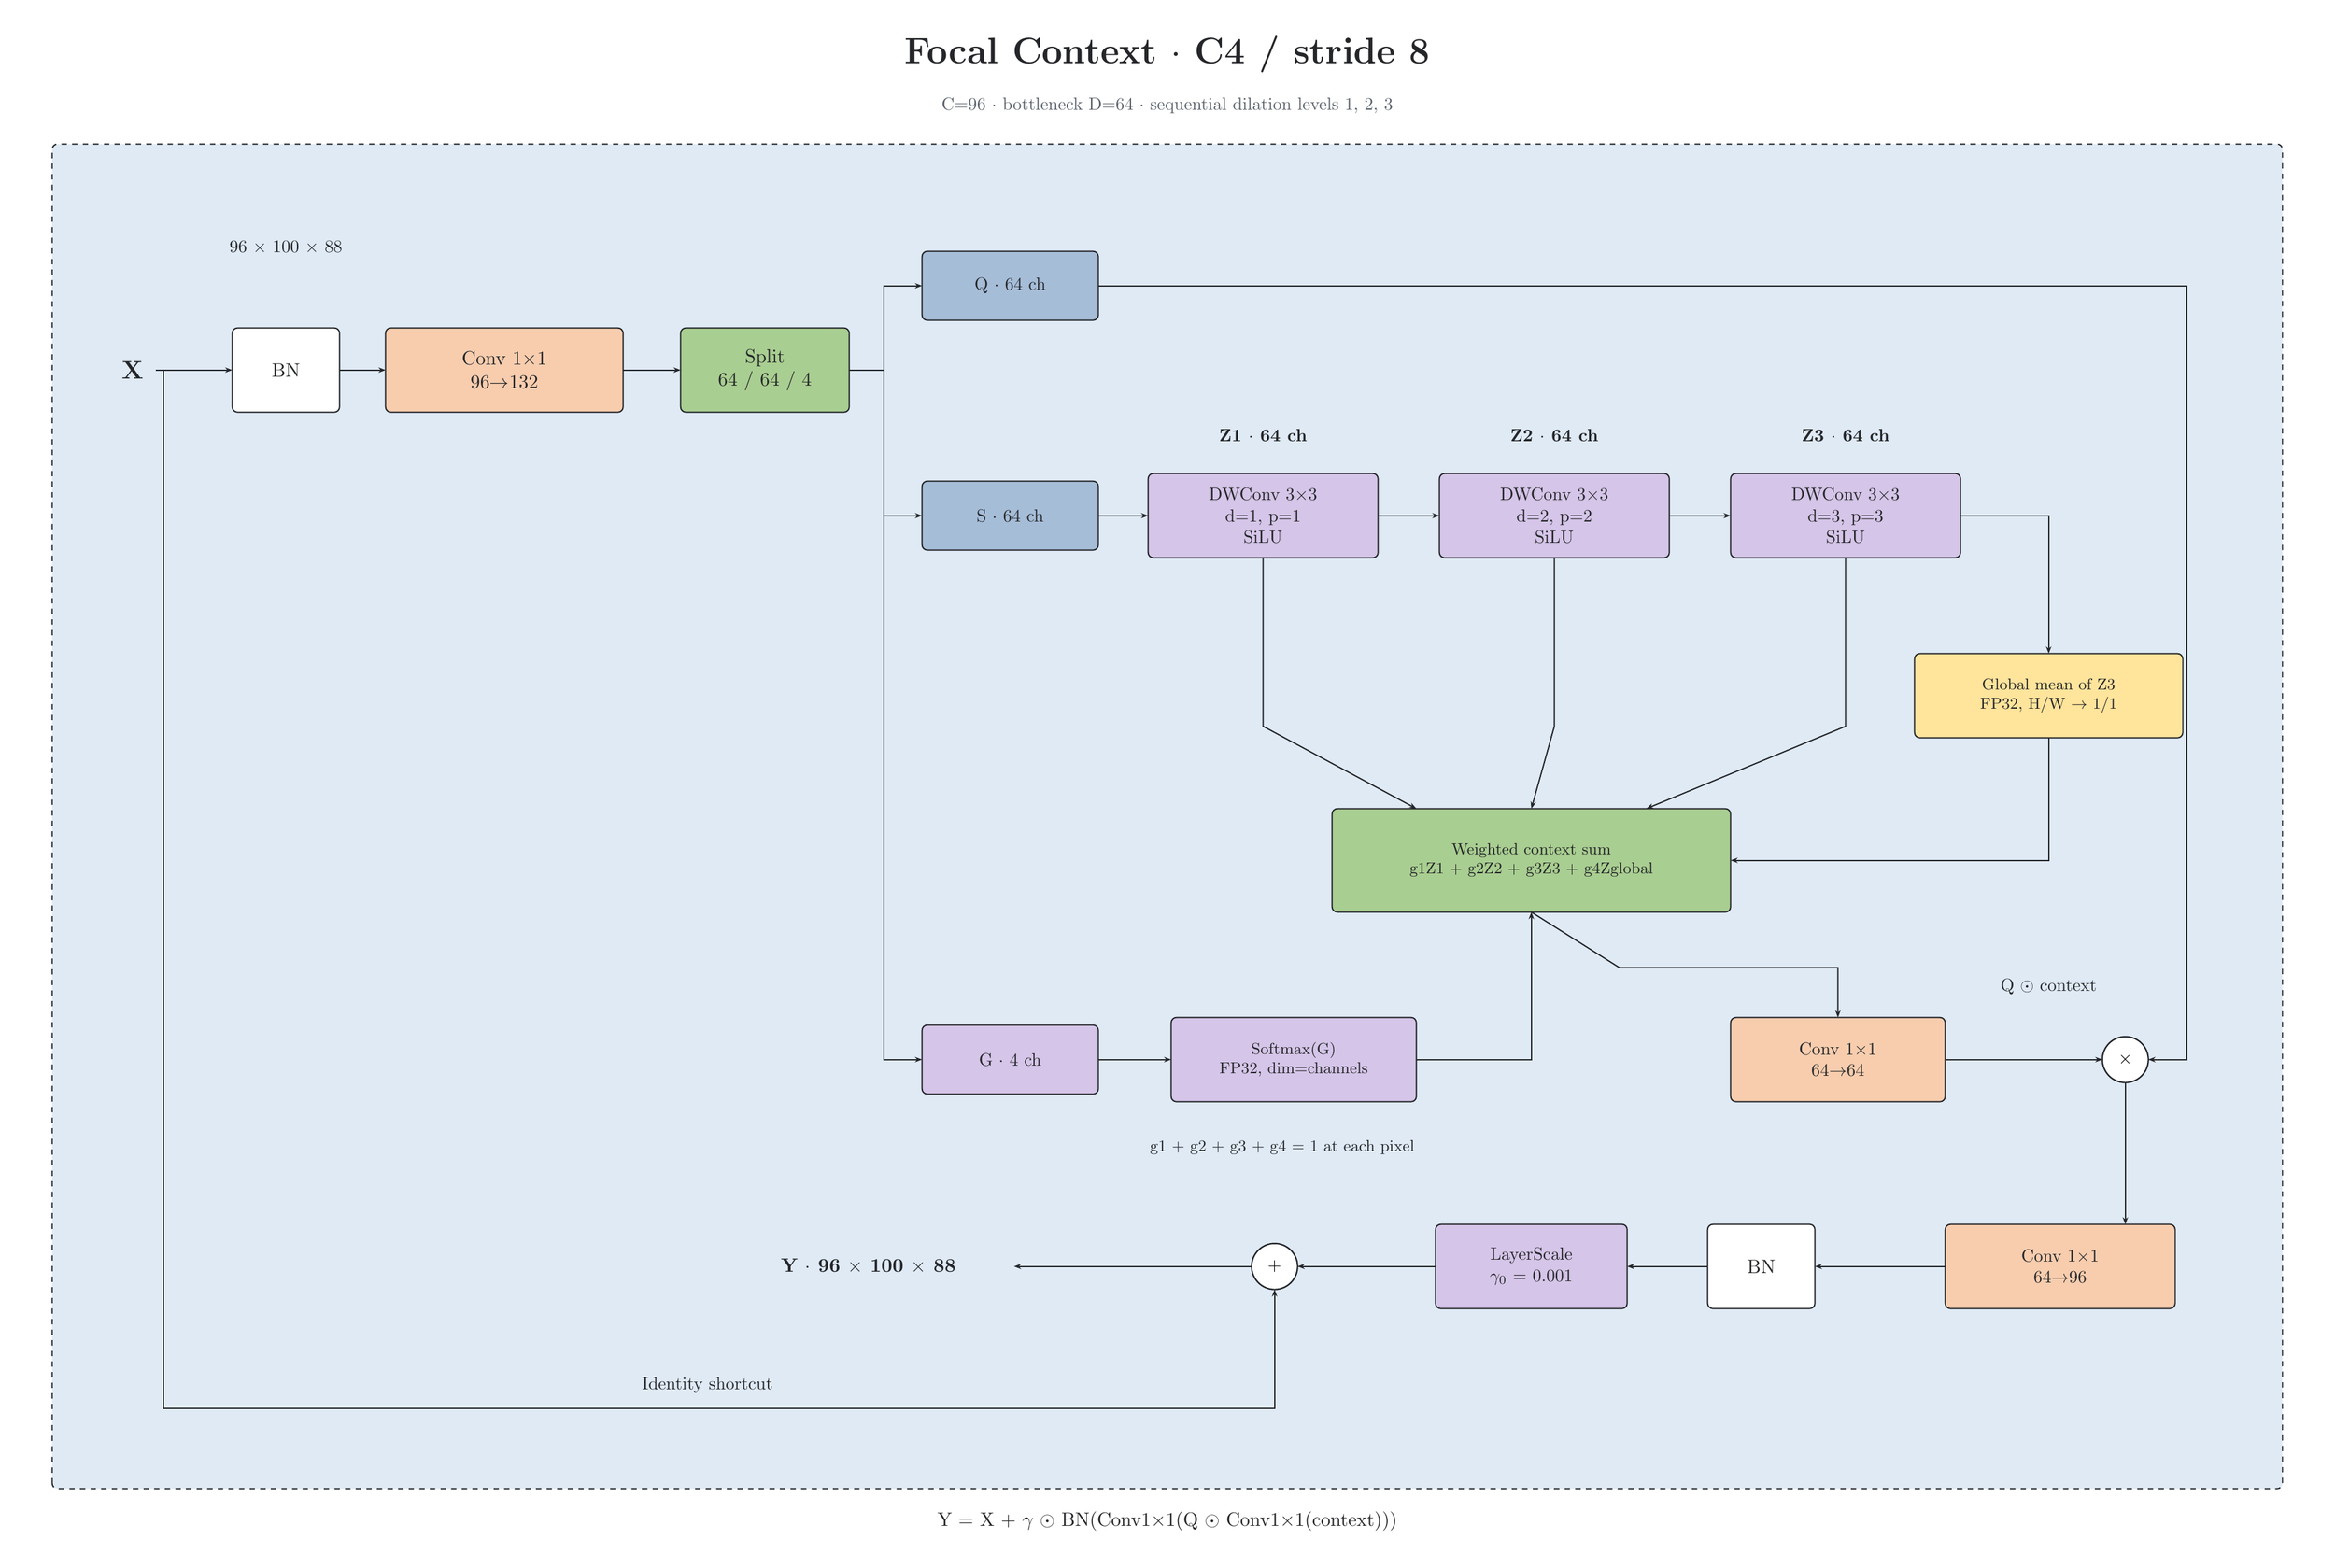
\begin{tikzpicture}[x=1.524cm,y=1.524cm,z={(0.9906cm,0.73152cm)}]
\path[use as bounding box] (0,0) rectangle (30,20);
\node[anchor=center,align=center,text=ink,font=\fontsize{20}{24.0}\selectfont \bfseries ] at (15.0,19.52) {Focal Context $\cdot$ C4 / stride 8};
\node[anchor=center,align=center,text=muted,font=\fontsize{10}{12.0}\selectfont ] at (15.0,18.85) {C=96 $\cdot$ bottleneck D=64 $\cdot$ sequential dilation levels 1, 2, 3};
\draw[draw=ink,fill=blue,rounded corners=3pt,line width=.7pt,dashed] (0.4499999999999993,0.8000000000000007) rectangle (29.55,18.35);
\node[anchor=west,align=left,text=ink,font=\fontsize{15}{18.0}\selectfont \bfseries ] at (0.8,17.85) {};
\node[anchor=center,align=center,text=ink,font=\fontsize{14}{16.8}\selectfont \bfseries ] at (1.5,15.4) {X};
\node[anchor=center,align=center,text=ink,font=\fontsize{10}{12.0}\selectfont ] at (3.5,17.0) {96 $\times$ 100 $\times$ 88};
\draw[-{Stealth[length=4pt]},draw=ink,line width=.7pt] (1.8,15.4) -- (2.8,15.4);
\draw[draw=ink,fill=white,rounded corners=3pt,line width=.7pt] (2.8,14.85) rectangle (4.2,15.950000000000001);
\node[anchor=center,align=center,text=ink,font=\fontsize{11}{13.2}\selectfont ] at (3.5,15.4) {BN};
\draw[-{Stealth[length=4pt]},draw=ink,line width=.7pt] (4.2,15.4) -- (4.8,15.4);
\draw[draw=ink,fill=peach,rounded corners=3pt,line width=.7pt] (4.8,14.85) rectangle (7.8999999999999995,15.950000000000001);
\node[anchor=center,align=center,text=ink,font=\fontsize{11}{13.2}\selectfont ] at (6.35,15.4) {Conv 1$\times$1\\96$\rightarrow$132};
\draw[-{Stealth[length=4pt]},draw=ink,line width=.7pt] (7.9,15.4) -- (8.65,15.4);
\draw[draw=ink,fill=green,rounded corners=3pt,line width=.7pt] (8.65,14.85) rectangle (10.85,15.950000000000001);
\node[anchor=center,align=center,text=ink,font=\fontsize{11}{13.2}\selectfont ] at (9.75,15.4) {Split\\64 / 64 / 4};
\draw[-{Stealth[length=4pt]},draw=ink,line width=.7pt] (10.85,15.4) -- (11.3,15.4) -- (11.3,16.5) -- (11.8,16.5);
\draw[draw=ink,fill=offset,rounded corners=3pt,line width=.7pt] (11.799999999999999,16.05) rectangle (14.1,16.95);
\node[anchor=center,align=center,text=ink,font=\fontsize{10}{12.0}\selectfont ] at (12.95,16.5) {Q $\cdot$ 64 ch};
\draw[-{Stealth[length=4pt]},draw=ink,line width=.7pt] (10.85,15.4) -- (11.3,15.4) -- (11.3,13.5) -- (11.8,13.5);
\draw[draw=ink,fill=offset,rounded corners=3pt,line width=.7pt] (11.799999999999999,13.05) rectangle (14.1,13.95);
\node[anchor=center,align=center,text=ink,font=\fontsize{10}{12.0}\selectfont ] at (12.95,13.5) {S $\cdot$ 64 ch};
\draw[-{Stealth[length=4pt]},draw=ink,line width=.7pt] (10.85,15.4) -- (11.3,15.4) -- (11.3,6.4) -- (11.8,6.4);
\draw[draw=ink,fill=purple,rounded corners=3pt,line width=.7pt] (11.799999999999999,5.95) rectangle (14.1,6.8500000000000005);
\node[anchor=center,align=center,text=ink,font=\fontsize{10}{12.0}\selectfont ] at (12.95,6.4) {G $\cdot$ 4 ch};
\draw[draw=ink,fill=purple,rounded corners=3pt,line width=.7pt] (14.75,12.95) rectangle (17.75,14.05);
\node[anchor=center,align=center,text=ink,font=\fontsize{10}{12.0}\selectfont ] at (16.25,13.5) {DWConv 3$\times$3\\d=1, p=1\\SiLU};
\draw[-{Stealth[length=4pt]},draw=ink,line width=.7pt] (14.1,13.5) -- (14.75,13.5);
\node[anchor=center,align=center,text=ink,font=\fontsize{10}{12.0}\selectfont \bfseries ] at (16.25,14.55) {Z1 $\cdot$ 64 ch};
\draw[draw=ink,fill=purple,rounded corners=3pt,line width=.7pt] (18.55,12.95) rectangle (21.55,14.05);
\node[anchor=center,align=center,text=ink,font=\fontsize{10}{12.0}\selectfont ] at (20.05,13.5) {DWConv 3$\times$3\\d=2, p=2\\SiLU};
\draw[-{Stealth[length=4pt]},draw=ink,line width=.7pt] (17.75,13.5) -- (18.55,13.5);
\node[anchor=center,align=center,text=ink,font=\fontsize{10}{12.0}\selectfont \bfseries ] at (20.05,14.55) {Z2 $\cdot$ 64 ch};
\draw[draw=ink,fill=purple,rounded corners=3pt,line width=.7pt] (22.35,12.95) rectangle (25.35,14.05);
\node[anchor=center,align=center,text=ink,font=\fontsize{10}{12.0}\selectfont ] at (23.85,13.5) {DWConv 3$\times$3\\d=3, p=3\\SiLU};
\draw[-{Stealth[length=4pt]},draw=ink,line width=.7pt] (21.55,13.5) -- (22.35,13.5);
\node[anchor=center,align=center,text=ink,font=\fontsize{10}{12.0}\selectfont \bfseries ] at (23.85,14.55) {Z3 $\cdot$ 64 ch};
\draw[draw=ink,fill=yellow,rounded corners=3pt,line width=.7pt] (24.75,10.6) rectangle (28.25,11.700000000000001);
\node[anchor=center,align=center,text=ink,font=\fontsize{9}{10.799999999999999}\selectfont ] at (26.5,11.15) {Global mean of Z3\\FP32, H/W $\rightarrow$ 1/1};
\draw[-{Stealth[length=4pt]},draw=ink,line width=.7pt] (25.35,13.5) -- (26.5,13.5) -- (26.5,11.7);
\draw[draw=ink,fill=green,rounded corners=3pt,line width=.7pt] (17.15,8.325) rectangle (22.35,9.675);
\node[anchor=center,align=center,text=ink,font=\fontsize{9}{10.799999999999999}\selectfont ] at (19.75,9.0) {Weighted context sum\\g1Z1 + g2Z2 + g3Z3 + g4Zglobal};
\draw[-{Stealth[length=4pt]},draw=ink,line width=.7pt] (16.25,12.95) -- (16.25,10.75) -- (18.25,9.675);
\draw[-{Stealth[length=4pt]},draw=ink,line width=.7pt] (20.05,12.95) -- (20.05,10.75) -- (19.75,9.675);
\draw[-{Stealth[length=4pt]},draw=ink,line width=.7pt] (23.85,12.95) -- (23.85,10.75) -- (21.25,9.675);
\draw[-{Stealth[length=4pt]},draw=ink,line width=.7pt] (26.5,10.6) -- (26.5,9) -- (22.35,9);
\draw[draw=ink,fill=purple,rounded corners=3pt,line width=.7pt] (15.049999999999999,5.8500000000000005) rectangle (18.25,6.95);
\node[anchor=center,align=center,text=ink,font=\fontsize{9}{10.799999999999999}\selectfont ] at (16.65,6.4) {Softmax(G)\\FP32, dim=channels};
\draw[-{Stealth[length=4pt]},draw=ink,line width=.7pt] (14.1,6.4) -- (15.05,6.4);
\draw[-{Stealth[length=4pt]},draw=ink,line width=.7pt] (18.25,6.4) -- (19.75,6.4) -- (19.75,8.325);
\node[anchor=center,align=center,text=ink,font=\fontsize{9}{10.799999999999999}\selectfont ] at (16.5,5.25) {g1 + g2 + g3 + g4 = 1 at each pixel};
\draw[draw=ink,fill=peach,rounded corners=3pt,line width=.7pt] (22.35,5.8500000000000005) rectangle (25.15,6.95);
\node[anchor=center,align=center,text=ink,font=\fontsize{10}{12.0}\selectfont ] at (23.75,6.4) {Conv 1$\times$1\\64$\rightarrow$64};
\draw[-{Stealth[length=4pt]},draw=ink,line width=.7pt] (19.75,8.325) -- (20.9,7.6) -- (23.75,7.6) -- (23.75,6.95);
\draw[fill=white,draw=ink,line width=.8pt] (27.5,6.4) circle (0.3);
\node at (27.5,6.4) {$\times$};
\draw[-{Stealth[length=4pt]},draw=ink,line width=.7pt] (25.15,6.4) -- (27.2,6.4);
\draw[-{Stealth[length=4pt]},draw=ink,line width=.7pt] (14.1,16.5) -- (28.3,16.5) -- (28.3,6.4) -- (27.8,6.4);
\node[anchor=center,align=center,text=ink,font=\fontsize{10}{12.0}\selectfont ] at (26.5,7.35) {Q $\odot$ context};
\draw[draw=ink,fill=peach,rounded corners=3pt,line width=.7pt] (25.15,3.1500000000000004) rectangle (28.15,4.25);
\node[anchor=center,align=center,text=ink,font=\fontsize{10}{12.0}\selectfont ] at (26.65,3.7) {Conv 1$\times$1\\64$\rightarrow$96};
\draw[-{Stealth[length=4pt]},draw=ink,line width=.7pt] (27.5,6.1) -- (27.5,4.25);
\draw[draw=ink,fill=white,rounded corners=3pt,line width=.7pt] (22.05,3.1500000000000004) rectangle (23.45,4.25);
\node[anchor=center,align=center,text=ink,font=\fontsize{11}{13.2}\selectfont ] at (22.75,3.7) {BN};
\draw[-{Stealth[length=4pt]},draw=ink,line width=.7pt] (25.15,3.7) -- (23.45,3.7);
\draw[draw=ink,fill=purple,rounded corners=3pt,line width=.7pt] (18.5,3.1500000000000004) rectangle (21.0,4.25);
\node[anchor=center,align=center,text=ink,font=\fontsize{10}{12.0}\selectfont ] at (19.75,3.7) {LayerScale\\$\gamma_0$ = 0.001};
\draw[-{Stealth[length=4pt]},draw=ink,line width=.7pt] (22.05,3.7) -- (21.0,3.7);
\draw[fill=white,draw=ink,line width=.8pt] (16.4,3.7) circle (0.3);
\node at (16.4,3.7) {+};
\draw[-{Stealth[length=4pt]},draw=ink,line width=.7pt] (18.5,3.7) -- (16.7,3.7);
\draw[-{Stealth[length=4pt]},draw=ink,line width=.7pt] (1.9,15.4) -- (1.9,1.85) -- (16.4,1.85) -- (16.4,3.4);
\node[anchor=center,align=center,text=ink,font=\fontsize{10}{12.0}\selectfont ] at (9,2.15) {Identity shortcut};
\draw[-{Stealth[length=4pt]},draw=ink,line width=.7pt] (16.1,3.7) -- (13,3.7);
\node[anchor=center,align=center,text=ink,font=\fontsize{11}{13.2}\selectfont \bfseries ] at (11.1,3.7) {Y $\cdot$ 96 $\times$ 100 $\times$ 88};
\node[anchor=center,align=center,text=ink,font=\fontsize{11}{13.2}\selectfont ] at (15,0.37) {Y = X + $\gamma$ $\odot$ BN(Conv1$\times$1(Q $\odot$ Conv1$\times$1(context)))};
\end{tikzpicture}
\end{document}
